% mainfile: ../../main.tex
\chapter{The \mjolnir measurement framework}\label{ch:exp:mjolnir}
\AutoLettrine{To} facilitate the optical experiments in \thispart, I wrote a software package that controls the measurement workflow and all other interactions with the setup described in \cref{part:setup}, \sidehref{https://git-ce.rwth-aachen.de/qutech/lab_software/python-mjolnir}{\mjolnir}~\cite{Hangleiter_mjolnir}.
The package is written in \python, is open source, and has a documentation as well as some rudimentary tests.\sidenote{
    Testing code interacting with hardware is notoriously difficult to achieve in an automated manner.
}
In this chapter, I lay out the goals and non-goals behind its development and briefly describe the design, features, as well as the typical workflow.

\section{Rationale}\label{sec:exp:mjolnir:rationale}
There exist various software solutions for measurement control, ranging from commercial (\eg, \sidehref{https://www.keysight.com/de/de/products/software/application-sw/labber-software.html}{Keysight Labber}) over open source (\sidehref{https://quantify-os.org/}{\package{quantify},} \sidehref{https://github.com/toolsforexperiments/labcore}{\package{labcore}}) to home-built (\sidehref{https://git-ce.rwth-aachen.de/qutech/frameworks/qool-tool}{\package{elicit},} \sidehref{https://github.com/qutech/qumada}{\qumada}).
While most of these frameworks attempt to achieve some degree of universality and not be tailored towards a specific type of experiment or setup, some bias always exists and most are geared towards fully electrical experiments.
On the other hand, software for optical experiments naturally exists as well, but it often suffers the same shortcomings coming from a different direction, and there is fairly little on offer for experiments at the interface of quantum optics and transport.
An added complication is the availability of drivers.
Striving for full automation of the setup, a number of different drivers are required given the complexity of the setup and the mix of electrical, optical, and mechanical instruments (\cref{part:setup}).
Thus, \qcodes forms a good basis for our specific needs due to its large driver coverage.
However, the wide array of physical instruments demands some level of abstraction to promote reproducibility and ease-of-use.
Furthermore, while \qcodes provides measurement functionality, their definition involves a large amount of repetitive setup code that needs to be duplicated for each measurement, invites errors, and degrades legibility.
The \sidehref{https://microsoft.github.io/Qcodes/api/dataset/index.html\#qcodes.dataset.dond}{\code{doNd}} functionality abstracts some of this away for multi-dimensional loops but is not flexible enough for our purposes.

By contrast, the experiments conducted in \thethesis do not place high demands on timing accuracy and measurement speed as typical \gls{pl} integration times are relatively long.
The software thus does not need to prioritize sophisticated triggering and pulsing logic required by qubit experiments.
Because the requirements are rather specific, \mjolnir is therefore single-minded.
It does not aspire to be suitable for applications other than the ones it is designed for.
The implementation is extremely biased towards the particular set of instruments in use in the lab and does not attempt to generalize to allow for different instruments to be used.
At the same time, it is designed to be modular, and different functionalities should be able to easily be replaced by other solutions.

\section{Instrument abstraction}\label{sec:exp:mjolnir:instruments}
\begin{figure*}
    \centering
    \begin{tikzpicture}[
    >=stealth,
    auto,
    box/.style={
        draw,
        rectangle,
        rounded corners,
        thick,
        align=center,
        inner sep=2mm,
%        drop shadow,
    },
    logical/.style={box, fill=RWTHmagenta25, text=RWTHmagenta100},
    physical/.style={box, fill=RWTHgreen25, text=RWTHgreen100},
    calibration/.style={box, fill=RWTHorange25, text=RWTHorange100},
    main/.style={circle, draw, thick, minimum size=12mm},
    sub/.style={circle, draw, thin, minimum size=6mm, font=\small},
    arrow/.style={thick}
]

    % Logical instruments
    \node[logical] (sam) {\mjolnirapidoc{mjolnir.instruments.logical_instruments.html\#mjolnir.instruments.logical_instruments.Sample}{\code{Sample}}};
    \node[logical, above left=2cm and 0.9cm of sam] (det) {\mjolnirapidoc{mjolnir.instruments.logical_instruments.html\#mjolnir.instruments.logical_instruments.DetectionPath}{\code{DetectionPath}}};
    \node[logical, above right=2cm and 0.9cm of sam] (exc) {\mjolnirapidoc{mjolnir.instruments.logical_instruments.html\#mjolnir.instruments.logical_instruments.ExcitationPath}{\code{ExcitationPath}}};

    % Physical instruments
    \node[physical] (dac) at ($(sam)+(195:2.5cm)$) {QDAC-II};
    \node[physical] (fridge) at ($(sam)+(240:2.5cm)$) {Triton 450};
    \node[physical] (magnet) at ($(sam)+(300:2.5cm)$) {Mercury iPS};
    \node[physical] (samdot) at ($(sam)+(345:2.5cm)$) {\dots};

    \node[physical] (spectrometer) at ($(det)+(165:3cm)$) {FHR1000};
    \node[physical] (ccd) at ($(det)+(195:3cm)$) {iDus 416};
    \node[physical] (tagger) at ($(det)+(225:2.5cm)$) {TimeTagger 20};
    \node[physical] (detdot) at ($(det)+(285:2cm)$) {\dots};

    \node[physical] (laser) at ($(exc)+(15:3cm)$) {M² Solstis};
    \node[physical] (shutter) at ($(exc)+(345:3cm)$) {MFF101/M};
    \node[physical] (ndfilter) at ($(exc)+(315:2.5cm)$) {K10CR1/M};
    \node[physical] (excdot) at ($(exc)+(255:2cm)$) {\dots};

    % Calibration handlers
    \node[calibration] (ccdcal) at ($(det)+(0cm,2cm)$) {\mjolnirapidoc{mjolnir.calibration.html\#mjolnir.calibration.CcdCalibrationHandler}{\code{CcdCalibrationHandler}}};
    \node[calibration] (power) at ($(exc)+(-2cm,1cm)$) {\mjolnirapidoc{mjolnir.calibration.html\#mjolnir.calibration.PowerCalibrationHandler}{\code{PowerCalibrationHandler}}};
    \node[calibration] (rejection) at ($(exc)+(+1cm,2cm)$) {\mjolnirapidoc{mjolnir.calibration.html\#mjolnir.calibration.RejectionFeedbackHandler}{\code{RejectionFeedbackHandler}}};

    % Arrows from physical to logical instruments
    \foreach \subnode in {dac,fridge,magnet,samdot}
        \draw[arrow, ->] (\subnode) -- (sam);
    \foreach \subnode in {spectrometer,ccd,tagger,detdot}
        \draw[arrow, ->] (\subnode) -- (det);
    \foreach \subnode in {laser,shutter,ndfilter,excdot}
        \draw[arrow, ->] (\subnode) -- (exc);

    % Arrows from logical instruments to calibration handlers
    \foreach \subnode in {ccdcal}
        \draw[arrow, ->] (det) -- (\subnode);
    \foreach \subnode in {power,rejection}
        \draw[arrow, ->] (exc) -- (\subnode);

    % Connections between logical instruments
    \draw[arrow, dashed, <->] (exc) -- (sam);
    \draw[arrow, dashed, <->] (sam) -- (det);
    \draw[arrow, dashed, <->] (det) -- (exc);

\end{tikzpicture}
    \caption[\imgsource{img/tikz/experiment/mjolnir_instruments.tex}]{
        Abstraction of physical instruments.
        \mjolnir defines three logical instrument classes (magenta) that represent different aspects of the experiment and group various physical instruments (green).
        Logical instruments expose various logical parameters that include communication with multiple physical instruments.
        \code{Sample} can be subclassed to suit the particular type of device under investigation.
        Calibration handlers (orange) are controlled by the logical instruments governing the optical path.
        Logical instruments are part of a \qcodes \code{Station} and can interact with each other as indicated by the dashed arrows.
    }
    \label{fig:exp:mjolnir:layout}
\end{figure*}

Central to the \mjolnir package is the abstraction of physical instruments into logical ones, thereby grouping logical functionality provided by different physical devices.
Take for instance the tunable \gls{cw} \tisalaser laser.
It is cooled by a Thermotek T225p chiller and pumped by a \pumplaser \gls{dpss} laser.
Behind its exit aperture, a \thorlabsflipper acts as a shutter, a \gls{nd} filter mounted on a \thorlabsrotator controls the output power, while a \thorlabspowermeter monitors the power at the optical head and an \rotatorcontroller controls the polarization state of the optical head.
Thus, seven different instruments from five different manufacturers are required to control the illumination state of the sample.
As a user, however, one would simply like to en- or disable the laser and set wavelength, power, and polarization configuration of the optical head.

To simplify and abstract away the particularities of the physical instruments providing control over parts of a user-facing parameter such as the excitation wavelength,\sidenote{
    For example, the power meter needs to be informed when changing the wavelength to keep the internal calibration up to date.
}
three logical instruments implemented as subclasses of the \qcodes \code{Instrument} class govern the experimental apparatus:
\begin{enumerate}\label{enm:logical_instruments}
    \item \label{itm:logical_instruments:exc}
        \code{ExcitationPath}.
        Controls all physical instruments related to illumination of the sample, including the white light source.
    \item \label{itm:logical_instruments:det}
        \code{DetectionPath}.
        Controls instruments related to the detection of radiation emitted by the sample, \ie, the spectrometer, \gls{ccd}, and photon counting card.
    \item \label{itm:logical_instruments:sam}
        \code{Sample}.
        Controls the \qdac voltage source, cryostat, and magnet, and implements a software representation of the \gls{dut}.
\end{enumerate}
\Cref{fig:exp:mjolnir:layout} shows a graph outlining the relationship between physical and logical instruments.
In the following, I give a brief overview of the functionalities comprised by these logical instruments.

\subsection{Excitation path}\label{subsec:exp:mjolnir:logical_instruments:exc}
\begin{marginfigure}
    \forestset{
    dir tree/.style={
        for tree={
            parent anchor=south west,
            child anchor=west,
            anchor=mid west,
            inner ysep=0pt,
            grow'=0,
            align=left,
            s sep=1ex,
            edge path={
                \noexpand\path [draw, \forestoption{edge}] (!u.parent anchor) ++(0.75em,0) |- (.child anchor)\forestoption{edge label};
            },
            font=\footnotesize\ttfamily,
            if n children=0{}{
                delay={
                    prepend={[,phantom, calign with current]}
                }
            },
            fit=band,
            before computing xy={
                l=1.25em
            }
        },
    }
}
\begin{forest}
    dir tree
    [
        [{\faIcon[regular]{folder} doc}]
        [{\faIcon[regular]{folder-open} src}
            [{\faIcon[regular]{folder-open} mjolnir}
                [{\faIcon[regular]{folder-open} config}
                    [{\faIcon[regular]{file-code} physical\_[\ldots].yaml}]
                    [{\faIcon[regular]{file-code} optical\_path.yaml}]
                    [{\faIcon[regular]{file-code} fig\_F10.yaml}]
                    [{\faIcon[regular]{file-code} \ldots}]
                ]
                [{\faIcon[regular]{folder-open} instruments}
                    [{\faIcon[regular]{file-code} \_\_init\_\_.py}]
                    [{\faIcon[regular]{file-code} logical\_[\ldots].py}]
                    [{\faIcon[regular]{file-code} physical\_[\ldots].py}]
                ]
                [{\faIcon[regular]{folder-open} measurements}
                    [{\faIcon[regular]{file-code} \_\_init\_\_.py}]
                    [{\faIcon[regular]{file-code} handler.py}]
                    [{\faIcon[regular]{file-code} measures.py}]
                    [{\faIcon[regular]{file-code} sweeps.py}]
                ]
                [{\faIcon[regular]{folder} parameters}
                    %[{\faIcon[regular]{file-code} \_\_init\_\_.py}]
                    %[{\faIcon[regular]{file-code} customized.py}]
                ]
                [{\faIcon[regular]{folder-open} plotting}
                    [{\faIcon[regular]{file-code} \_\_init\_\_.py}]
                    [{\faIcon[regular]{file-code} live\_view.py}]
                    [{\faIcon[regular]{file-code} plot\_nd.py}]
                ]
                [{\faIcon[regular]{file-code} \_\_init\_\_.py}]
                [{\faIcon[regular]{file-code} calibration.py}]
                %[{\faIcon[regular]{file-code} \_version.py}]
                %[{\faIcon[regular]{file-code} helpers.py}]
                [{\faIcon[regular]{file-code} \ldots}]
            ]
        ]
        [{\faIcon[regular]{file-code} main.py}]
        [{\faIcon[regular]{file-code} pyproject.toml}]
        [{\faIcon[regular]{file-code} \ldots}]
    ]
\end{forest}

    \caption[\imgsource{img/tikz/experiment/mjolnir_tree.tex}]{
        Source tree structure of the \mjolnir package.
        Logical \qcodes instruments and parameters are defined in the \code{instruments} and \code{parameters} modules, respectively.
        Instruments are configured using \code{yaml} files located in a \code{config} subdirectory.
        The \code{measurements} module provides classes for the abstraction of measurements using \qcodes underneath.
        Live plots of instrument data as well as a plot function for multidimensional measurement data are defined in the \code{plotting} module.
        \code{calibration.py} contains routines for power, \acrshort{ccd}, and excitation rejection calibrations.
        The \code{main.py} file is a code cell-based script that serves as the entrypoint for measurements.
    }
    \label{fig:exp:mjolnir:tree}
\end{marginfigure}

As already outlined above, the \code{ExcitationPath} object controls everything related to the illumination of the sample.
The \code{active_light_source} parameter switches between laser, white light, and no illumination.
Turning on the laser comprises enabling the chiller, switching on the pump laser, waiting for it to ramp up, and asserting the wavelength lock is acquired.
For safety reasons, confirmation by the user that they are physically in the lab is required.
Furthermore, the \code{ExcitationPath} instrument implements setting the excitation power by means of a calibration of the \gls{nd} filter, see \cref{sec:exp:mjolnir:calibration}.
Since the output power of the laser varies depending on wavelength, the object furthermore provides a \code{wavelength_constant_power} parameter that automatically recalibrates the power once a new wavelength is set.
Finally, it manages the state of the automatic excitation rejection control, see \cref{sec:exp:mjolnir:calibration}.

\subsection{Detection path}\label{subsec:exp:mjolnir:logical_instruments:det}
The \code{DetectionPath} object is responsible for the optical analysis.
Chiefly, it manages the \thespectrometer spectrometer and provides convenient shorthands for selecting grating (\code{active_grating}) and exit port (\code{active_detection_path}, either \code{"ccd"} or \code{"apd"}).
It handles initialization of the spectrometer and the \gls{ccd} including the \gls{ccd} cooler and oversees calibration of the \gls{ccd} pixel-to-wavelength relation, see \cref{sec:exp:mjolnir:calibration}.
From the \gls{ccd} calibration and its pixel size, the dispersion at the imaging plane of the currently selected grating can be obtained, allowing the user to set the monochromator bandwidth of the spectrometer in terms of a wavelength window rather than the more abstract exit slit width.

\subsection{Sample}\label{subsec:exp:mjolnir:logical_instruments:sam}
The \code{Sample} class initializes the \qdac \gls{dac} and magnet power supply.
Mainly, though, it serves as an abstraction of the actual \gls{dut} and its \enquote{control knobs} such as gates.
Users implement subclasses for different sample designs.
As the samples we are concerned with in \thethesis, I discuss the main implementation, \code{TrapSample}, representing samples with exciton traps.
On a single sample, there are any number of traps consisting of one or both sets of top and bottom \enquote{central} and \enquote{guard} gates.
Each trap is implemented as a \qcodes \code{InstrumentModule}, \code{Trap}, that is part of a \code{ChannelList}.
The currently active trap (\ie, the one currently in focus by the microscope) is selected by the \code{active_trap} parameter and accessible through the \code{trap} property of the \code{TrapSample} object.
A \code{Trap} exposes the virtual gate parameters\sidenote[][*4]{
    Using the \qdac's built-in \hidelinkhref{https://qcodes.github.io/Qcodes_contrib_drivers/api/generated/qcodes_contrib_drivers.drivers.QDevil.html\#qcodes_contrib_drivers.drivers.QDevil.QDAC2.Arrangement_Context}{\code{Arrangement_Context}} virtual gate functionality.
}
\code{difference_mode} and \code{common_mode} (see \cref{subsec:exp:observations:pl:qcse}) as the difference and sum of top and bottom gate voltages, respectively, as well as the unmodified top and bottom gate voltage and corresponding leakage current parameters.
\Gls{dac} channels are mapped to their corresponding \code{Trap} parameters using \code{yaml} configuration files specific to each sample and hosted in a separate repository.

\section{Calibrations}\label{sec:exp:mjolnir:calibration}
\mjolnir implements three automatic calibration procedures in the classes \code{CcdCalibrationHandler}, \code{PowerCalibrationHandler}, and \mintinline[breaklines,breakbefore=FH]{python}{RejectionFeedbackHandler} (see \cref{fig:exp:mjolnir:layout}).
As their names suggest, these handle calibration of the \gls{ccd} pixel-to-wavelength conversion, the power transmission through the rotatable \gls{nd} filter, and the waveplate and polarizer angles for optimal laser rejection, respectively.

\subsection{CCD calibration}\label{subsec:sec:exp:mjolnir:calibration:ccd}
Because the dispersion of the spectrometer gratings depends to a small degree on wavelength, the calibration function converting horizontal \gls{ccd} screen pixels into wavelengths needs to be updated for every central wavelength selected using the grating.
In principle, this requires measuring the position of several reference wavelengths on the \gls{ccd} screen and fitting a polynomial of second or third degree.
As the tunable \gls{cw} laser is coupled to a wavelength meter with built-in calibration lamp (HighFinesse WS6), it lends itself naturally as a source of the reference wavelength.
In practice, the deviation from an established calibration function is usually small enough that simply shifting the center pixel (that is, the zeroth-order polynomial term) suffices for reasonably small wavelength ranges of tens of nanometers.
The \code{CcdCalibrationHandler} implements three different calibration schemes specified as the \code{ccd_calibration_update_mode} parameter of the \code{DetectionPath} instrument:
\begin{enumerate}
    \item \code{"full"}.
        The pixel position of the maximum intensity of nine equidistant wavelengths centered around the grating central wavelength and spread out over the entire range of the \gls{ccd} screen ($\sim\qty{45}{\nano\meter}$ for the \qty{600}{gr\per\milli\meter} grating and $\sim\qty{9}{\nano\meter}$ for the \qty{1800}{gr\per\milli\meter} grating) is measured sequentially and fitted to a third-degree polynomial.
    \item \code{"fast"}.
        The laser is set to the grating central wavelength and the zeroth-order coefficient of the previous calibration polynomial is shifted by the pixel distance between the peak and the horizontal center of the \gls{ccd} screen.
    \item \code{"dirty"}.
        The zeroth-order coefficient of the calibration polynomial is shifted by the difference in nominal grating and laser wavelengths.
\end{enumerate}
By default, the \code{"dirty"} mode is enabled as it does not require any grating moves or wavelength changes and is therefore the fastest.
Rather than recalibrating, old calibration data can also be loaded from disk if it is not older than a user-specified date.
Finally, note that the spectrometer grating motor also requires occasional recalibration.
Both the coefficient of linearity (converting motor steps to selected central wavelength) and the offset in motor steps can change over time.
Currently, this calibration is not automated but is instead compensated for by shifting the central wavelength on the \gls{ccd} screen.
In principle, the driver for the \thespectrometer spectrometer implements all necessary functionality for automating the calibration procedure already.

\subsection{Power calibration}\label{subsec:sec:exp:mjolnir:calibration:power}
The \gls{nd} filter\sidenote{
    Thorlabs NDC-25C-4~\cite{ThorlabsNDC-25C-4}.
}
mounted on the \thorlabsrotator rotation stage has a continuously variable \gls{od} (\cref{eq:setup:optics:od}) of \numrange{0.04}{4.0}, which depends quite sensitively on the wavelength.
In order to allow reliably setting a specified excitation power at any excitation wavelength, the \mjolnir package automates the calibration of the filter angle against transmitted power.
Two modes are implemented, \code{"full"} and \code{"fast"}.
In the former mode, the transmitted power is sampled at a given angular interval and the resulting data fitted using a quadratic smoothing spline.
\Cref{fig:exp:mjolnir:power_calibration} shows a typical measurement and spline fit at \qty{795}{\nano\meter}.
The specified power is then set by inverting the spline and evaluating at the given power.

\begin{marginfigure}
    \centering
    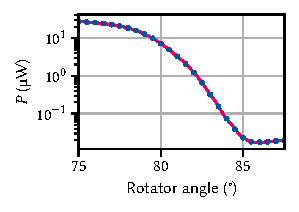
\includegraphics{img/pdf/experiment/power_calibration}
    \caption[\imgsource{img/py/experiment/calibration.py}]{
        Power calibration using the continuously variable \acrshort{nd} filter.
        Error bars from statistics are too small to see.
        Magenta line is a quadratic smoothing spline.
    }
    \label{fig:exp:mjolnir:power_calibration}
\end{marginfigure}

As performing the full calibration is quite time-consuming and furthermore the inversion not fully reliable, the \code{"fast"} calibration update mode sets the rotator angle by performing a noisy optimization.
Here, first the last valid full calibration is loaded and its spline scaled to the current power level.
Then, the residual sum of squares between the target power and the power meter reading is minimized using the \code{noisyopt} package~\cite{Mayer2016} with the starting value given by the angle predicted by the rescaled calibration spline.

\subsection{Rejection feedback}\label{subsec:sec:exp:mjolnir:calibration:rejection}
The excitation rejection by means of cross-polarization extinction has already been discussed in \cref{subsec:setup:optics:coupling:rejection}.
As shown there, the \gls{od} achieved by cross-polarizing the excitation beam with the analyzer mounted in the detection path reaches a maximum close to \num{6} and is extremely sensitive to small variations in the angles of the \quarterwave- and \halfwave-plates controlling polarization state.
Close to the optimum, the \gls{od} is well-described by a parabola as function of those angles, with a second-order polynomial coefficient on the order of \qty[per-mode = symbol]{-0.15}{\per\square\milli\txtdegree}.
Since the optics including the waveplates display chromatic dispersion, the excitation rejection needs to be re-optimized whenever the laser wavelength is changed, and the exponential angular dependence of the transmitted intensity places high demands on the dynamic range of the photo-detector used for measurement.
Therefore, the reflected laser intensity is measured with the \gls{apd} signal digitized by the \tagger on the side exit port of the spectrometer.\sidenote{
    The signals from both \glspl{apd} are combined to achieve the best \gls{snr}, see \cref{part:setup}.
}
The \taggershort can reliably cover a count rate range from \qtyrange{1e2}{1e6}{cps}, compared to the \theccd \gls{ccd} covering only \qtyrange{1e3}{1e5}{cps}.

In the \mjolnir package, the calibration is then carried out as a bivariate noisy minimization using \package{noisyopt}~\cite{Mayer2016}.
Upon initialization the power is set to a small value to avoid overexposing the detectors.
Then, the spectrometer is set to select the laser wavelength, the side exit port is selected, and the optimization over the \quarterwave- and \halfwave-angles is run within conservatively set bounds of $[\qty{-2.5}{\degree}, \qty{2.5}{\degree}]$, which has been found to be a good compromise of robustness and convergence speed.
A caching mechanism stores the optimal angles together with the current wavelength, which serves as a starting guess upon subsequent calibration runs.
The calibration is quite tedious and time-consuming for several reasons.
Chiefly, moving the waveplate angles is slow simply because it is a mechanical movement, and optimizers typically do not take into account the distance between subsequent sample points, potentially resulting in unnecessarily inefficient exploration of the parameter space.
Incorporating a penalty on the sample distance into the optimization algorithm would hence improve the convergence speed.
Additionally, due to vibrations in the cryostat (\cref{ch:setup:vibrations}), the \gls{rms} intensity of the back-scattered laser is large -- and larger the closer the excitation rejection is to its optimal value\sidenote{
    The count rate can vary by up to a factor of two with the frequency of the \gls{ptr} pulses.
} -- and thus requires long averaging times for a robust measurement.
Finally, the algorithm outlined above fails when the starting guess is too far away from the optimum, such as when the new wavelength is on the order of tens of \unit{nm} away from the previously optimized one.
A good -- albeit time-consuming -- strategy is then to incrementally update the wavelength.

\section{Measurement routines}\label{sec:exp:mjolnir:measurement}
Measurements in \mjolnir use the \qcodes infrastructure for data acquisition and storage.
To abstract away code for repetitive setup and teardown tasks, the user interacts with a \code{MeasurementHandler} object through the \code{measure()} method.
The class can be subclassed to customize the aforementioned tasks for different types of experiments (such as those that involve illumination with the laser and detection with the \gls{ccd}, \code{LaserCcdMeasurementHandler}), or add default parameters to every measurement (such as leakage currents or the laser power).
A measurement's independent parameters are passed to \code{measure()} as instances of a \code{Sweep} class which completely determines the measurement structure.
\code{Sweep} objects support syntactic sugar for concatenation (\code{@}), nesting (\code{|}), and parallelization (\code{&}).
Dependent parameters (those that should be measured) can be simple parameters or instances of a \code{Measure} class.\sidenote{
    Besides some optimization for measurements of parameters delegating from the same physical parameter, the latter exists mostly for (primitive) live plotting.
}
The state of external parameters, that is, parameters that are not varied or measured during a measurement, can be defined for the duration of the measurement using the \code{parameter_contexts} argument, a mapping from \qcodes parameters to valid values thereof.
This uses the \code{Parameter.set_to()} context manager to set the parameters to the given values before the measurement starts and restore their original values upon exit in a controlled manner, allowing users to ensure their device is in a well-defined state.
Custom setup and teardown tasks can furthermore be specified through the \code{add_before_run} and \code{add_after_run} arguments, respectively.

\begin{listing}[htpb]
    \begin{py}
        from mjolnir.measurement.handler import LaserCcdMeasurementHandler
        from mjolnir.measurement.sweeps import GridSweep
        from mjolnir.measurement.measures import Measure

        handler = LaserCcdMeasurementHandler(station)

        # excitation_path, sample are instances of the ExcitationPath and
        # TrapSample classes, respectively
        power_sweep = GridSweep(excitation_path.power_at_sample,
                                rng=(5e-9, 5e-7), num_points=11,
                                spacing='geom')
        gate_sweep = GridSweep(sample.trap.central_difference_mode,
                               rng=(-2, -1), num_points=51))

        # two-dimensional sweep over power and gate voltage
        sweeps = power_sweep | gate_sweep
        # keep track of the MXC temperature
        measures = sample.fridge.T8

        dataset = handler.measure(
            sweeps,
            measures,
            parameter_contexts={
                sample.trap.central_common_mode: -1,
                detection_path.central_wavelength: 825,
            },
            exposure_time=2
        )
    \end{py}
    \caption[\mjolnir measurement workflow]{
    Setup and measurement workflow using the \mjolnir package.
        \code{station} is a \qcodes \code{Station} object managing the instruments.
        The \code{sweeps} object describes a nested loop on whose inner iteration the difference mode parameter of the trap's central gate is swept over a linear grid and on whose outer iteration the laser power, adjusted for the \acrlong{bs} ratio, is swept over a logarithmically spaced grid.
        No dependent parameters (\code{Measure} objects) need to be explicitly specified as the \code{LaserCcdMeasurementHandler} measures the \gls{ccd} spectrum as well as laser power and leakage currents of the swept gates by default.
        The \code{parameter_contexts} argument is used to set the spectrometer wavelength to \qty{825}{\nano\meter} and the common mode voltage of the active trap to \qty{-1}{\volt}.
        The \code{exposure_time} argument is passed through to the \code{initialize} method, where it is used to set up the \gls{ccd} for acquisition.
    }
    \label{lst:exp:mjolnir:workflow}
\end{listing}

A typical workflow for a \gls{pl} measurement using laser and \gls{ccd} is sketched in \cref{lst:exp:mjolnir:workflow}.
The \code{MeasurementHandler} object automatically takes care of, among other things, arming the \gls{ccd}, acquiring a background image in the dark, and opening the laser shutter for the duration of the measurement.
Acquired data is saved to the \qcodes database, but a helper function exporting to the \xarray \code{Dataset} format is available.
Saved together with the data are a snapshot of the \qcodes \code{Station} as well as arbitrary custom metadata.
More details and examples on the measurement functionality can be found in the \sidehref{https://qutech.pages.git-ce.rwth-aachen.de/lab_software/python-mjolnir/}{documentation.}
Lastly, I note that the measurement functionality in \mjolnir is independent of the instrument abstraction and calibration logic and as such could be replaced or augmented with minimal effort by that of other \qcodes-based frameworks such as \package{quantify} or \package{labcore} to make use of their infrastructure.
I leave this option for future work.

\section{Plotting}\label{sec:exp:mjolnir:plotting}
\begin{figure*}
    \centering
    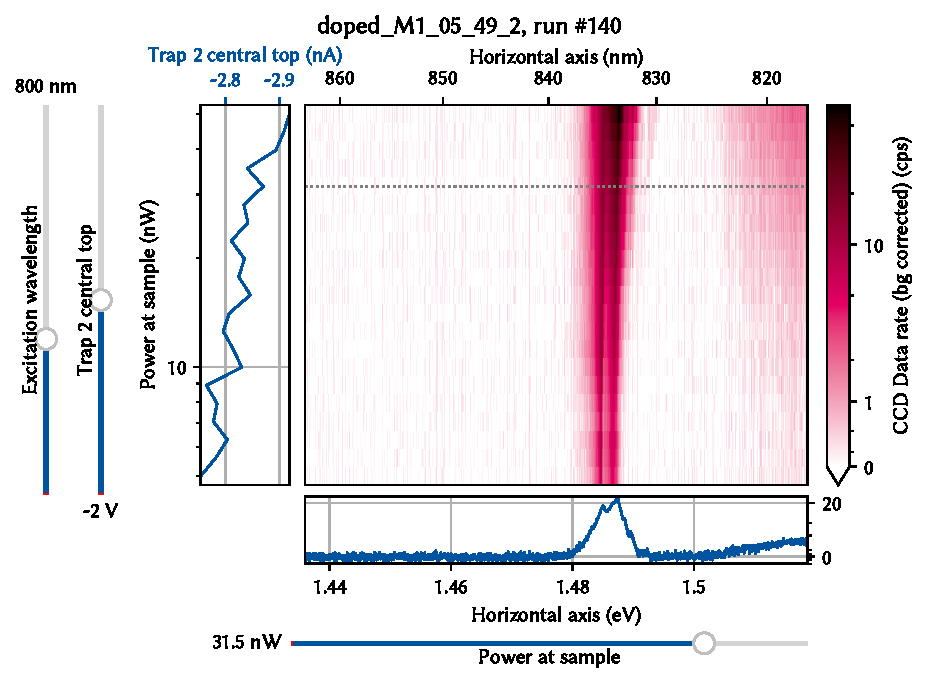
\includegraphics{img/pdf/experiment/plot_nd}
    \caption[\imgsource{img/py/experiment/pl.py}]{
        The \code{plot_nd()} plot window.
        The bottom panel, enabled by default, shows a horizontal line cut through the 2D data of the main panel whose $y$-value can be set with the adjacent slider widget.
        The left panel shows the leakage currents of gates that participate in the sweep and, if measured, the laser power.
        A vertical slider widget is added for each data dimension not displayed on the $x$ or $y$ axis of the main plot.
        The figure title shows the sample as well as the measurement identifiers assigned by \qcodes.
    }
    \label{fig:exp:mjolnir:plot_nd}
\end{figure*}

Optical measurements using \mjolnir often produce multi-dimensional datasets by virtue of the default parameter measured, the \gls{ccd} spectrum, being vector-valued or \emph{batched}.
To visualize such datasets with more than two dimensions, \mjolnir provides the \code{plot_nd()} function that plots 2D slices through the data as a false-color image and generates interactive slider widgets that allow users to modify the slice coordinates.
This facilitates interactively exploring large datasets and recognizing trends present in the data beyond two dimensions.
\Cref{fig:exp:mjolnir:plot_nd} shows an exemplary plot window for a four-dimensional data set obtained from a \gls{ccd} measurement sweeping laser wavelength, power, and a gate voltage, with \cref{lst:exp:mjolnir:plot_nd} showing the code necessary to produce the plot.

\begin{listing}
    \begin{py}
        import matplotlib as mpl
        from mjolnir.plotting import plot_nd

        fig, axes, sliders = plot_nd(
            dataset_or_run_id=140, vertical_target='power_at_sample',
            yscale='log', norm=mpl.colors.AsinhNorm(vmin=0),
            fig_kw=dict(figsize=(6.33585, 4.6))
        )
    \end{py}
    \caption[\texttt{plot_nd()} example]{
        Code to produce the plot shown in \cref{fig:exp:mjolnir:plot_nd}.
        If \code{dataset_or_run_id} is an integer, the currently connected \qcodes database is queried for this run identifier.
        Otherwise, it should be an \xarray \code{Dataset}.
    }
    \label{lst:exp:mjolnir:plot_nd}
\end{listing}

The plotting functionality is implemented using \matplotlib.
While not the most performant library, its flexibility in decorating and customizing plots as well as scaling data, such as the $\asinh$-scale normalization used in \cref{fig:exp:mjolnir:plot_nd}, made it the preferred choice.
To nonetheless improve the responsivity of the interactive elements, the plotted artists are \emph{blitted}\sidenote{
    Blitting refers to storing constant backgrounds of raster graphics and only redrawing changing elements.
    See the \matplotlib \href{https://matplotlib.org/stable/users/explain/animations/blitting.html}{documentation}.
}
using the \code{qutil.plotting.BlitManager} class from the \qutil library~\cite{Hangleiter_qutil}.
The data variable to be shown in the main panel can be selected with the \code{array_target} argument, which accepts a string and chooses the closest match in the dataset since the full parameter names are often a bit unwieldy.
Similarly, the coordinates to be plotted on the $x$- and $y$-axes are selected with the \code{horizontal_target} and \code{vertical_target} arguments, respectively.

In addition to plotting measurement data, \mjolnir implements live plotting of instrument data leveraging the \code{qutil.plotting.live_view} module.
Since most instruments do not support multiple concurrent connections, switching control between the \python console and the \gls{gui} program provided by the manufacturer can often be tedious.\sidenote{
    For instance, the \gls{ccd} \gls{gui}, Andor Solis, by default disables the thermoelectric cooler when exiting the program.
}
Thus, making use of their continuous data acquisition functionality is prohibitively time-consuming, but at the same time optical experiments frequently call for live observation of instrument data, for example when aligning the optics.
Live plotting is currently implemented for three different instruments and corresponding parameters; the \thorlabspowermeter power meter (power reading), the \theccd \gls{ccd} (spectrum or image), and the \tagger counting card (count rate(s)).
Data acquisition is executed in a background thread while the plot, implemented in \matplotlib, currently runs in the main thread, and hence does not update while the interpreter is blocked.
In principle, though, the \code{live_view} module also supports plotting in a separate process, making a multiprocessing implementation straightforward.
Interactive \gls{gui} elements in the \matplotlib figure allow for pausing and automatically rescaling the data.\sidenote{
    These two features can also be activated with the \textsc{space} and \textsc{r} keys.
}
Since for the \gls{ccd} data acquisition runs using the \emph{run till abort} mode of the device and as such continuously, the instrument is blocked for the duration of the live plot and it therefore needs to be closed before starting a measurement.
By contrast, the power meter and \taggershort parameters are simply queried regularly in sequential mode and can hence in principle remain open and running while performing measurements.